\subsection{Definition and motivation}

According to \citep{Hothorn.2006} an algorithm for recursive partitioning is called unbiased when, under the conditions of the null hypothesis of independence between a response $y$ and feature $\textbf{x}_{1},...\textbf{x}_{p}$ the probability of selecting feature $\textbf{x}_{j}$ is $1/p$ for all $j = 1,...,p$ regardless of the measurement scales or number of missing values. 

This definition may be surprising at first, since if there is no dependency between the target and the features, one would not want to perform a split anyway and would try to prevent this through appropriate pruning procedures.
However, the idea behind this is that if, in the case of independence, a feature with, for example, a large number of possible split points is selected more frequently as a splitting variable than a feature with a smaller number of split points, the former could also be incorrectly selected more frequently as a splitting variable if there is a dependency on the response for the second feature.
\citep{Loh.2014}

In the discussion on the Paper Fifty Years of Classification and Regression Trees of \citep{Loh.2014}, Carolin Strobl's statement on selection bias is therefore very clear:
\vspace{0.5cm}


{\par\centering \textit{"One should think that the results shown here [...] are so clear that any statistically educated person should never
want to use a biased recursive partitioning algorithm again."}\par}
\vspace{0.5cm}

So if SLIM is the only biased algorithm, it would have to be discarded immediately according to this statement. However, this will be investigated in detail in the following.



\subsection{Simulation independence scenarios}
In order to empirically investigate whether the four algorithms presented actually correspond to the respective groups (biased and unbiased) using the definition of \citet{Hothorn.2006}, two different simulation were carried out.

In the first scenario only numerical features are used, whereas in the second scenario numerical features and additionally one binary and two categorical features are considered.

\paragraph{Independence numeric\\}
The data in the first scenario is defined as follows:
\begin{itemize}
    \item $\textbf{x}_{1}, \textbf{x}_{2} \sim U(0,1)$
    \item $\textbf{x}_3$ uniformly distributed on the set $\{0, 0.1,..., 0.9, 1\}$
    \item $\textbf{x}_4$ uniformly distributed on the set $\{0, 0.01,..., 0.99, 1\}$
    \item $y \sim N(0,1)$
    \item sample size $n = 1000$
    \item 1000 simulation runs
\end{itemize}

The resulting frequencies are shown in Figure \ref{fig:selection_bias_independence_numeric} and are consistent with the expectations. SLIM clearly prefers to select features with a higher number of split points and therefore is biased. The other three methods seem to  select all four features about the same number of times.

\begin{figure}[!htb]
    \centering
    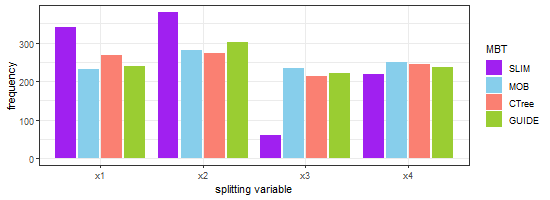
\includegraphics[width=10cm]{Figures/simulations/chapter_4_selection_bias/selection_bias_general/independence_numerical.png}
    \caption{Simulated frequencies of selected splitting features for scenario independence numeric}
    \label{fig:selection_bias_independence_numeric}
\end{figure}



\paragraph{Selection bias independence mixed \newline} 
In the second scenario, the data is simulated as follows:
\begin{itemize}
    \item $\textbf{x}_{1}, \textbf{x}_{2} \sim U(0,1)$ 
    \item $\textbf{x}_3$ uniformly distributed on the set $\{0, 0.1,..., 0.9, 1\}$ 
    \item $\textbf{x}_4  \sim Bern(0.5)$ 
    \item $\textbf{x}_5$ uniformly distributed on 5 factor levels (15 possible splits) 
    \item $\textbf{x}_6$ uniformly distributed on 8 factor levels (128 possible splits) %stirling number of second kind    
    \item $y \sim N(0,1)$
    \item sample size $n = 1000$
    \item 1000 simulation runs
\end{itemize}

The addition of categorical features in this scenario results in a different picture for the frequencies, as shown in Figure \ref{fig:selection_bias_independence_mixed}. Although the numerical variables are chosen with approximately equal frequency in the so-called "unbiased" methods, there are large deviations in the binary and categorical variables especially for MOB and CTree, which calls the designation "unbiased" into question. 
A possible explanation for this selection bias could be that due to the large number of parameters that have to be estimated for the categorical features in the modelling step, random dependencies to the target variable are already caught well in the model  and therefore these variables are used less frequently as splitting variables.


In \citep{Hothorn.2006} the unbiasedness of CTree is empirically investigated for cases, in which a strict separation between regressor variables and partitioning variables is kept. Therefore, the result shown here should not principally question the label, but it does not seem appropriate when there is an overlap or, as in our case, even congruence between the two roles.


\begin{figure}[!htb]
    \centering
    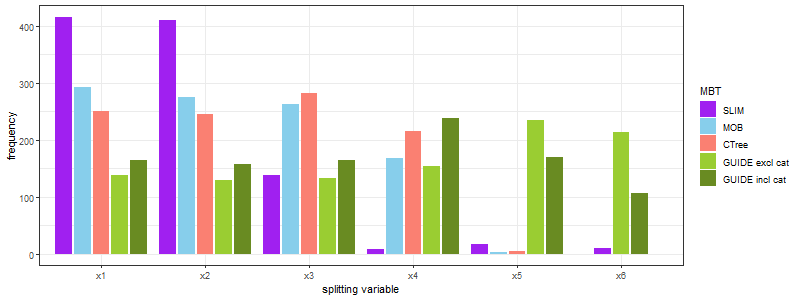
\includegraphics[width=14cm]{Figures/simulations/chapter_4_selection_bias/selection_bias_general/independence_mixed.png}
    \caption{Simulated frequencies of selected splitting features for scenario independence mixed}
    \label{fig:selection_bias_independence_mixed}
\end{figure}

For GUIDE two different variants were evaluated in this scenario. "GUIDE excl cat" corresponds to the original version, in which categorical features are only used as splitting and not as regressor variables. In "GUIDE incl cat", on the other hand, the categorical features are also used as regressors. The fact that the frequencies of the categorical variables are smaller in "GUIDE incl. cat" could be explained analogously to the selection bias of MOB and CTree.

The binary feature $\textbf{x}_4$ is almost never chosen as a splitting variable with SLIM, in contrast to the other variables. However, this can be attributed to the selection bias in numerical features with different numbers of split points, as the binary variable can be seen as numerical variable with only one possible split point. What is more interesting is that the numerical variable $\textbf{x}_2$ with 10 possible split points is chosen by SLIM much more frequently as splitting variable than the variable $\textbf{x}_6$ with 128 possible splits, so that the bias cannot be determined by the number of possible splits alone.

The difference between the categorical ($\textbf{x}_5$ and $\textbf{x}_6$) and the numerical variables can probably be explained in a similar way as with the other methods, but in reverse. With SLIM, the potential split is executed first and then models in the child nodes are fitted.  If a numerical feature is used as partitioning variable, the parameters for all factor levels are estimated in both child models, whereby random dependencies with $y$ can be modelled very accurately. If, on the other hand, splitting is done according to a categorical variable, only a subset of the factor levels can be used for modelling in both child nodes.






As a possible correction approach for the selection bias in SLIM, I investigated how the number of quantiles considered as potential split points affects the selection bias and the performance (mean square error) of SLIM. The simulation setup and results are shown in the appendix \ref{app:selection_bias_correction}. In summary, although selection bias can be reduced for numerical variables in the case of an independent target variable, this correction can lead to unpredictable biases if interactions are actually present. For this reason, the approach is not recommended. 
For all simulations in this chapter, each unique value was seen as a potential split point for SLIM.






\subsection{Simulation interaction scenarios} \label{selection_bias_interactions}
While so far only the frequencies with which different feature types are selected in the case of independence were shown, it is empirically investigated in the following which feature types the different MBT algorithms tend to select when interactions are actually present.
Four different scenarios are examined for this. These are, in a sense, pair comparisons of different feature types. In all scenarios, the data generating process consists of two pairs of interactions, whereby the interactions have the same strength. Each pair consists of a numerical variable that enters linearly into the interaction and another variable that splits the linear effect into two subgroups.
In all four scenarios the numerical variables which define the linear effect are 
 $\textbf{x}_{2}, \textbf{x}_{4} \sim U(0,1)$ .

The features $\textbf{x}_{1}$ and $\textbf{x}_{3}$ are responsible for the subgroups. They are uniformly distributed on sets, which are given in Table \ref{tab:selection_bias_interaction}, as well as the data generating processes.

\begin{table}[!htb]
    \centering
    \begin{tabular}{llll}
        \hline
        scenario & $\textbf{x}_1$ & $\textbf{x}_3$ & $f(\textbf{x})$\\
        \hline
        numerical vs numerical & $[0,1]$ &  $\{0, 0.1,..., 0.9, 1\}$ & $\mathbb{1}_{(\textbf{x}_1 \leq  mean(\textbf{x}_1))}\textbf{x}_2  +  \mathbb{1}_{(\textbf{x}_3 \leq  mean(\textbf{x}_3))}\textbf{x}_4 $ \\
        binary vs categorical & $\{0,1\}$ &  $\{a,b,c,d,e,f\}$ & $\mathbb{1}_{(\textbf{x}_1 = 0)}\textbf{x}_2  +  \mathbb{1}_{(\textbf{x}_3 \in \{a,b,c\})}\textbf{x}_4 $ \\
        numerical vs binary & $[0,1]$ & $\{0,1\}$ & $\mathbb{1}_{(\textbf{x}_1 \leq  mean(\textbf{x}_1))}\textbf{x}_2  +  \mathbb{1}_{(\textbf{x}_3 = 0)}\textbf{x}_4$ \\
        numerical vs categorical & $[0,1]$ & $\{a,b,c,d,e,f\}$ & $\mathbb{1}_{(\textbf{x}_1 \leq  mean(\textbf{x}_1))}\textbf{x}_2  +  \mathbb{1}_{(\textbf{x}_3 \in \{a,b,c\})}\textbf{x}_4$ \\
        \hline
    \end{tabular}
    \caption{Simulation scenarios selection bias interaction}
    \label{tab:selection_bias_interaction}
\end{table}





All experiments are repeated 1000 times. The error terms are set to $\epsilon \sim N(0, 0.1 \cdot sd(f(\textbf{x}))$ and the data generating processes are $y = f(\textbf{x}) + \epsilon$.



First of all, there is the question of how selection bias should be defined in these scenarios. Transferring the definition from the independence case, one possibility would be to require that the frequency of being selected as a split variable for all features is 1/4.  However, this does not take into account that splits according to $\textbf{x}_1$  and $\textbf{x}_3$ , i.e. according to the split features that define the subgroups, produce a considerable greater improvement in performance than splits according to the smooth features $\textbf{x}_2$  and $\textbf{x}_4$. If $\textbf{x}_1$  and $\textbf{x}_3$  are chosen preferentially, one should not regard this as selection bias but as a good splitting strategy to get the smallest and best performing trees possible. What could be expected from an unbiased procedure, however, is that both interaction pairs are chosen equally often for the first split.



\begin{figure}[!htb]
    \centering   
    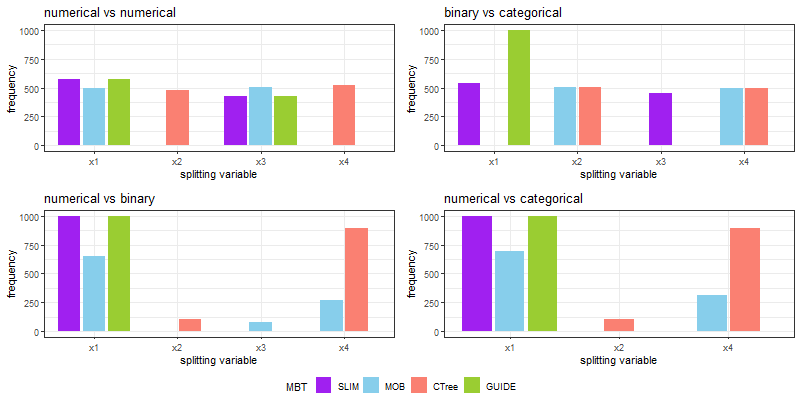
\includegraphics[width = 16cm]{Figures/simulations/chapter_4_selection_bias/selection_bias_general/interactions.png}
    \caption{Simulated frequencies of selected splitting features for the four interaction scenarios}
    \label{fig:selection_bias_interactions}
\end{figure}

Figure \ref{fig:selection_bias_interactions} shows the frequencies of the first selected split variable in each scenario for each MBT. It can be seen that in none of the scenarios and for none of the MBTs the results seem to be equally distributed among all four features. 
As a general rule, it is noticeable that SLIM and GUIDE always prefer the subgroup-defining variables ($\textbf{x}_1$  and $\textbf{x}_3$) for splitting, while CTree always prefers the smooth variables. For MOB, the behaviour varies depending on the feature type.

In Scenario "numerical vs numerical", the distribution for MOB and CTree is at least evenly distributed between the two interactions pairs. One could therefore speak of unbiasedness here. However, while CTree only uses the linear features $\textbf{x}_2$ and $\textbf{x}_4$ as the first split variable, MOB splits according to the subgroup-defining features, which is preferable in practice.
In GUIDE and SLIM, only the features $\textbf{x}_1$ and $\textbf{x}_3$ are selected, but there seems to be a preference for the variable $\textbf{x}_1$, which has a larger number of potential split points.


In the scenario "binary vs categorical", the distribution between the two interaction pairs seems to be roughly equal for SLIM, MOB and CTree. In contrast to the first scenario, MOB does not split according to the subgroup-defining variables but with regard to the linear features.
In GUIDE, only the binary variable is selected, so there is a clear preference for the binary variable over the categorical variable.

In the remaining scenarios, a strong selection bias is evident in all MBTs. SLIM, for example, gives considerable preference to numerical subgroup-defining variables over binary and categorical variables.





Obviously, these scenarios do not represent a complete overview of possible interactions. However, since MBTs can show their strengths especially in the presence of subgroup-specific maineffects (i.e. good interpretability through small trees but good performance at the same time), only such scenarios are compared here. These simulation results should sensitise to the fact that in certain cases variables could only be selected as splitting variables because they have certain properties and not because their share in an interaction is actually the largest, even with the so-called unbiased methods.

Finally it should be noted that even if selection bias is present in the independence case, this does not necessarily lead to the wrong variable being selected for splitting. In particular, this can often be prevented by pruning. However, as far as could be observed here, selection bias is very difficult to control or predict and should therefore always be considered when using these algorithms.





%\textbf{Test for selection bias:} $\chi^2$ goodness of fit test\\
%H0: the probabilities of the population are all equal (or are equal to an assumed probability distribution p)





